\documentclass[twocolumn]{article}
\usepackage[utf8]{inputenc}
\usepackage[skip=6pt, indent=0pt]{parskip}
\usepackage{graphicx}
\usepackage{tikz}
\usetikzlibrary{automata, positioning, arrows}

\title{CS 460 {-} Compilers}
\author{Arian Izadi}
\date{Spring 2024}

\begin{document}

\maketitle

\section{Languages}

Syntax is the rules for what a syntactically correct program looks like.
Semantics is the meaning of a program.

When does it matter the order of evaluation (right to left vs left to right)?
When the code has side effects, an example of this is postfix vs prefix increment (a++ vs ++a).

Compilers for a language L, move from front end $\to$ intermediate representation $\to$ back end.

\begin{itemize}
  \item Front end: Lexical Analysis, Syntax Analysis, and Semantic Analysis
  \item Intermediate: Intermediate Code
  \item Back end: Optimizer and Code Generation
\end{itemize}

\subsection{Lexical Analysis \& Scanning}

Lexical analysis, a scanner, is the process of converting a stream of characters into a stream of tokens.

\begin{enumerate}
  \item Find all terminals in the grammar.
  \item Write the Scanner.
        \begin{enumerate}
          \item Do we use a DFA, NFA, or PDA{?}
          \item Look at token types. All tokens can be expressed by a regular expression.
                \begin{enumerate}
                  \item Symbols: Semicolon, commas, etc.
                  \item Keywords: for, while, etc.
                  \item Variables: x, y, etc.
                  \item Numbers: 1, 3.14, 0{x}64, etc.
                \end{enumerate}
        \end{enumerate}
\end{enumerate}

\pagebreak

\paragraph*{Chomsky Language Hierarchy}

\begin{itemize}
  \item Type 0: Unrestricted (Turing Machines)
  \item Type 1: Context Sensitive
  \item Type 2: Context Free (PDA)
  \item Type 3: Regular Expressions (NFA, DFA)
\end{itemize}

Both RE and CFG have 1 non-terminal on the left of any combination of terminals and non-terminals on the right.

\textbf{Example 1:}

$S \to X$
\hfill
$X \to aXb | d$
\hfill
not regular: $a^n d b^n$

\textbf{Example 2:}

$S \to X$
\hfill
$X \to aX | b$
\hfill
regular: $a^* b$

\textbf{Example 3:}

$S \to X$
\hfill
$X \to aY | \epsilon$
\hfill
$Y \to bX$
\hfill
regular: $(ab){^*}$

An NFA for recognizing tokens, construct NFA for each construct of RE\@.

$\mathcal{E}$:

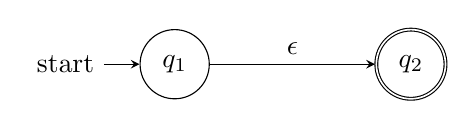
\begin{tikzpicture}[>=stealth, node distance=3cm, on grid, auto]
  \node[state, initial] (q1) {$q_1$};
  \node[state, accepting, right=of q1] (q2) {$q_2$};
  \path[->] (q1) edge node {$\epsilon$} (q2);
\end{tikzpicture}

$a \epsilon \Sigma$:

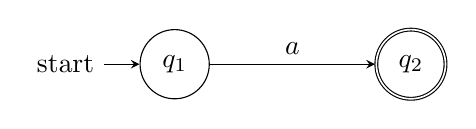
\begin{tikzpicture}[>=stealth, node distance=3cm, on grid, auto]
  \node[state, initial] (q1) {$q_1$};
  \node[state, accepting, right=of q1] (q2) {$q_2$};
  \path[->] (q1) edge node {$a$} (q2);
\end{tikzpicture}

\pagebreak

% $s | t$:

% \begin{tikzpicture}[>=stealth, node distance=2cm, on grid, auto]
%   \node[state, initial] (q1) {$q_1$};
%   \node[state, right=of q1] (q2) {$q_2$};
%   \node[state, accepting, right=of q2] (q3) {$q_3$};
%   \node[state, below=of q2] (q4) {$q_4$};

%   \path[->] (q1) edge node[above] {$\epsilon$} (q2);
%   \path[->] (q2) edge node[above] {$\epsilon$} (q3);
%   \path[->] (q1) edge node[left] {$\epsilon$} (q4);
%   \path[->] (q4) edge node[right] {$\epsilon$} (q3);
% \end{tikzpicture}


Any RE can be turned into an NFA using these rules.
If all the tokens of a language are represented by RE's, $r_1, \dots, r_n$.
Create an NFA for each RE\@.


\section{Parsing}

\subsection{Types of Parsers}

\begin{itemize}
  \item $LL(k)$ $-$ leftmost derivation
        \begin{itemize}
          \item (Hard Explain) Always develop the leftmost non terminal in a sentential form.
          \item Above means: Start at the start symbol and work towards the input.
        \end{itemize}
  \item $LR(k)$ $-$ rightmost derivation
        \begin{itemize}
          \item Reverse rightmost derivation.
          \item Above means: Start at input and work backwards to the start symbol.
        \end{itemize}
\end{itemize}

\paragraph*{Types of $LL(k)$ parsers:}

\begin{itemize}
  \item $LL(0)$ $-$ No look ahead and no left recursion.
  \item $LL(1)$ $-$ One look ahead and no left recursion.
  \item $LL(k)$ $-$ $k$ look ahead and no left recursion.
\end{itemize}

% example
\paragraph*{Example 1: $a^* b^*$}

% capital epsilon

$\delta(a^* b^*) = {\mathcal{\epsilon}, a, b, aa, ab, bb, \dots}$

$S \to A$
\hfill
$A \to aA | B$
\hfill
$B \to bB | \mathcal{\epsilon}$

Try $w = aabb$:

$S \to_{LM} A \to_{LM} aA \to_{LM} aaA \to_{LM} aaB \to_{LM} aabB \to_{LM} aabbB \to_{LM} aabb$

What if B could generate strings starting with an $a$?

$S \to A$
\hfill
$A \to aA | B$
\hfill
$B \to bB | a | \mathcal{\epsilon}$

Try $w = aabb$:

It cannot be parsed by an $LL(1)$ parser.

\pagebreak

\paragraph*{A is not $LL(1)$ when}
\begin{itemize}
  \item $\exists w_1 \in \lambda (\alpha _1)$ or $\exists w_2 \in \lambda (\alpha _2)$
  \item $w_1 = aw_1$ or $w_2 = aw_2$
\end{itemize}

\paragraph*{Example 2:}
A set representing tokens that a sentential form can start with: Call it $FIRST(\alpha)$

\begin{enumerate}
  \item $\mathcal{\epsilon}: $ FIRST ($\mathcal{\epsilon}$) = $\{\mathcal{\epsilon}\}$
  \item $a\in \Sigma: $ FIRST ($a$) = $\{a\}$
  \item a mixed string: $Y = Y_1 Y_2 \dots Y_n$
        \begin{enumerate}
          \item FIRST ($Y_1 \dots Y_n$) $\supseteq$ FIRST ($Y_1$) \ $\{\mathcal{\epsilon}\}$
          \item if $\mathcal{\epsilon} \exists$ FIRST ($Y_1$):
                \begin{enumerate}
                  \item $Y_1, Y_2, \dots, Y_n \to \mathcal{\epsilon}$
                  \item $Y_1, Y_2, \dots, Y_n \to Y_2, \dots, Y_n$
                \end{enumerate}
        \end{enumerate}
\end{enumerate}


\paragraph*{Example 3:}

$X \to X_1 | \dots | X_m$

FIRST ($X$) = FIRST ($X_1$) $\cup$ FIRST ($X_2$) $\cup \dots \cup$ FIRST ($X_m$)

% \begin{center}
%   \begin{tabular}{|c|c|}
%     FIRST (A) & FIRST (B) \\
%     \hline
%     4         & 5         \\
%     \hline
%     7         & 8         \\
%     \hline
%     9         & 10
%   \end{tabular}
% \end{center}

\paragraph*{Example 4: }
General Case

For $A \to \alpha _1 | \alpha _2 | \dots | \alpha _n$

if $\exists i, j$ such that $i \neq j$ and FIRST ($\alpha _i$) $\cap$ FIRST ($\alpha _j$) $\neq \emptyset$ then $A$ is not $LL(1)$.

\textbf{MUST BE DONE PAIRWISE, only needs to exist one pair to not be $LL(1)$.}

$\forall i, j: i \neq j \string^ (1 <= i, j <= n): FIRST (\alpha _i) \cap FIRST (\alpha _j) = \emptyset$ then $A$ is probably (necessary, but not sufficient) $LL(1)$.

\paragraph*{Example 5:}
General Case

For $A \to \alpha _1 | \alpha _2 | \dots | \alpha _n$

\vdots

$A_m \to \alpha _{m1} | \alpha _{m2} | \dots | \alpha _{mn_m}$

\newpage

\textbf{Example 6:}

$A \to B | C$

\vdots

$B \to \dots$

$C \to \dots$

FIRST ($B$) = \{a, b\}
FIRST ($C$) = \{c, f\}

$w = a \beta$ where $a \in \Sigma$ and $\beta \in \Sigma ^*$

* $a$ is the lookahead token.

$A \to _{LM} B \to _{LM} aX$

* $aX$ matches $a \beta$, so we can derive $\beta$ from $X$.

\subsection{Grammar Transformation}

\subsubsection{Left vs Right Recursion}

$A \to Aa | b$

$\delta(A) = \{b, ba, baa, \dots\} = ba^*$

FIRST ($A$) = \{b\}
FIRST ($Aa$) = \{b\}

* Both have $b \to $ and is not $LL(1)$.

* Just make it right recursive.

$A \to bA'$

$A' \to aA' | \mathcal{\epsilon}$

\textbf{In General:}

$A \to A \alpha _1 | A \alpha _2 | \dots | A \alpha _n | \beta _1 | \beta _2 | \dots | \beta _m$

$\delta(A) = (B _1 | \dots | B _n) (\alpha _1 | \dots | \alpha _n) $

$A \to \beta _1 A' | \dots | \beta _m A'$

$A' \to \alpha _1 A' | \dots | \alpha _n A' | \mathcal{\epsilon}$

\textbf{Example 4.6:}

$E \to E + b | b$ similar to $A \to A \alpha | \beta$

$E \to bE'$

$E' \to + bE' | \mathcal{\epsilon}$

\newpage

\textbf{Example 4.7:}

$E \to E + b | E - c | b | C$ similar to $A \to A \alpha _1 | A \alpha _2 | \beta _1 | \beta _2$

$E \to bE' | CE'$

$E' \to + bE' | - cE' | \mathcal{\epsilon}$

\subsubsection{Common Subexpressions}

\textbf{Example 4.8:}

$A \to abC | abD$

* is this LL (1)? 

No, because FIRST ($abC$) $\cap$ FIRST ($abD$) $\neq \emptyset$.

* if we change it to $A \to abA'$ and $A' \to c | D$, then it is LL (1).

* is this LL (1)? 

Only if FIRST ($c$) $\cap$ FIRST ($D$) $= \emptyset$.

\textbf{For the following:}

$A \to A _1 | \dots | A _n$

Let $\alpha$ be the longest common prefix of $A _1, \dots, A _n$ such that $A _i = \alpha A' _i$. 
Then $A \to \alpha A'$ and $A' \to A _1 | \dots | A _n$.

\subsubsection{Grammar Ambiguity}

Definition: A grammar is ambiguous if there exists a string $w$ such that there are two or more different parse trees for the same string.

$A \to aA | bA | c$ with $w = ababc$.

$A \to aA \to abA \to abaA \to ababA \to ababc$

\textbf{Simple Example:}

$A \to aA | a | \mathcal{\epsilon}$

\textbf{Example 4.9:}

$E \to E + E | E - E | id$ is this ambiguous?

Yes, because $id + id - id$ can be parsed as $(id + id) - id$ or $id + (id - id)$.

\newpage

\textbf{PHASE 2 ADVICE:} AST is never the answer to the left hand side, use a subclass of it.

What if we want +, -, *, /?

$E \to E + E | E - E | E * E | E / E | id$

Consider $id + id * id$.

* is higher precedence than +, so $id + (id * id)$.

When dealing with precedence, the lower precedence should be higher in the parse tree.

$E \to E + T | E - T | T$

$T \to T * F | T / F | F$

$F \to id | (E)$

* The bracket is the highest precedence.

* This is also bad because it is left recursive.

\textbf{Eliminate Left Recursion:}

$E \to TE'$

$E' \to + TE' | - TE' | \mathcal{\epsilon}$

$T \to FT'$

$T' \to * FT' | / FT' | \mathcal{\epsilon}$

$F \to id | (E)$


\subsection{Recursive Descent Parsing}

$A \to B | C$

$B \to b | \epsilon$

$C \to c$

* lookahead = \$

$A \to B \to \epsilon$

\begin{verbatim}
  parse_x();
  parse_y();
  match('a');
  parse_z();
\end{verbatim}

\newpage

\begin{verbatim}
  parse_A() {
    if (lookahead == 'b') {
      parse_B();
    } else if (lookahead == 'c') {
      parse_C();
    } else {
      // will not check error vs epsilon
      // this is a problem
      // if none of alpha i are epsilon
    }
  }
\end{verbatim}


\end{document}